\documentclass[11pt]{scrartcl}

\usepackage{fullpage}
\usepackage{mdwlist}
\usepackage[english]{babel}
\usepackage[hidelinks]{hyperref}
\usepackage{graphicx}

% Define a \blankpage command to generate boilerplate.
\newcommand*{\blankpage}{%
\clearpage
\vspace*{\fill}
\centerline{This page intentionally left blank.}
\vspace{\fill}
\clearpage}

% Make every \section{} start on a new page.
\let\stdsection\section
\renewcommand\section{\newpage\stdsection}

\title{PikYak Requirements Document}
\subtitle{Version 1, draft}
\author{
    George Hilliard (gh403) \\
    Collin Kelso (chk59) \\
    Kevin Stephens (ks910)
}
\date{2014 October 9}

\hypersetup{pdftitle={PikYak Requirements Document},
            pdfauthor={George Hilliard; Collin Kelso; Kevin Stephens}}

\begin{document}

\pagenumbering{roman}

\maketitle

\blankpage

\tableofcontents

\blankpage

\pagenumbering{arabic}

\section{Introduction}
    \subsection{Purpose}
        The purpose of this Requirements Document is to specify the software requirements of PikYak, an anonymous picture sharing social media platform.
        The document will help to define the concept and functionality of PikYak for development.

    \subsection{Definitions, Acronyms, and Abbreviations}
        \begin{description*}
            \item[post:] A message, containing only a single picture, submitted to the public PikYak server for other users to view.

            \item[up-vote:] A single positive vote that users can give to a post to signify that they enjoy the content.

            \item[down-vote:] A single negative vote that users can give to a post to signify that they do not enjoy the content.

            \item[score:] The value of the sum of a post's downvotes subtracted from the sum of its upvotes.
                          This measure provides a rough indication of how popular a post is.

            \item[conversation:] A grouping of posts that are made in reply to one another.
                                 Creating a new post either creates a new conversation or replies to an existing one.
        \end{description*}

    \subsection{References}
        IEEE Std. 830-1998, IEEE Recommended Practice for Software Requirements Specifications, Institute for Electrical and Electronic Engineers, Piscataway, New Jersey, 1998.

\section{System Overview}
    \subsection{Purpose}
        PikYak will be an anonymous picture sharing application that allows users to exchange images with other users that are local to each other.  The application will allow users to comment, upvote, and downvote images.
    \subsection{Use Case Diagram}
        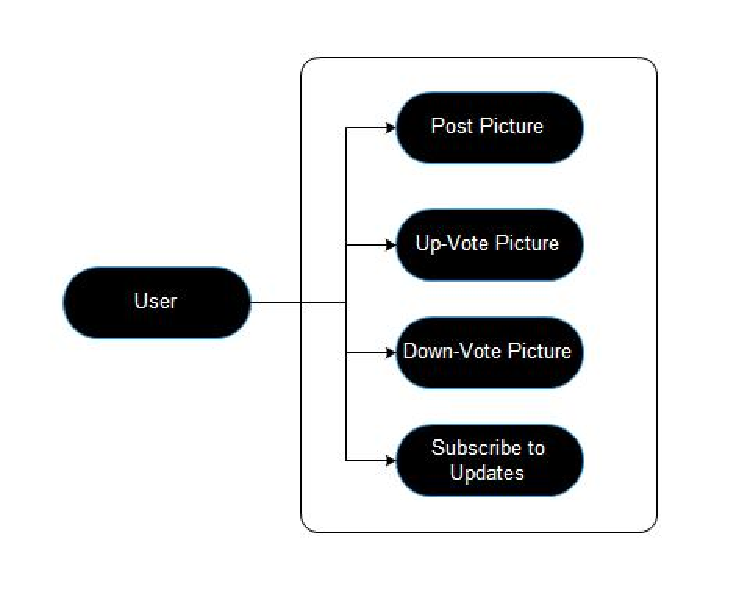
\includegraphics{useCase}

\section{Specific Requirements}
    \subsection{Post Picture (Required)}
        \subsubsection{Description}
            The user would like to create a conversation by uploading a picture.
        \subsubsection{Actors}
            \begin{itemize}
                \item User
            \end{itemize}
        \subsubsection{Steps}
            \begin{enumerate}
                \item The user launches the PikYak client application on their device.
                \item The application displays a list of recent conversations, with a thumbnail of the most recent image in each conversation. In the top right there is an icon to create a conversation.
                \item The user taps the icon.
                \item The camera opens and the user is allowed to take a picture.
                \item The application shows a preview of the picture asks the user to confirm that they want to post it.
                \item The image is submitted and a conversation is created.
            \end{enumerate}
    
    \subsection{Up-vote Picture (Required)}
        \subsubsection{Description}
            The user would like to up-vote a conversation they like.
        \subsubsection{Actors}
            \begin{itemize}
                \item User
            \end{itemize}
        \subsubsection{Steps}
            \begin{enumerate}
                \item The user launches the PikYak client application on their device.
                \item The application displays a list of recent conversations, with a thumbnail of the most recent image in each conversation.
                \item The user will choose one of the conversations by tapping it.
                \item The application will display the recently posted pictures in the conversation, with an up-arrow and a down-arrow.
                \item The user will tap the up-arrow.
                \item The application will immediately advise the server of the user's action, and all other clients' devices will be updated immediately.
                \item Each post's score will be displayed next to the post.
            \end{enumerate}

    \subsection{Down-vote Picture (Required)}
        \subsubsection{Description}
            The user would like to down-vote a conversation they dislike.
        \subsubsection{Actors}
            \begin{itemize}
                \item User
            \end{itemize}
        \subsubsection{Steps}
            \begin{enumerate}
                \item The user launches the PikYak client application on their device.
                \item The application displays a list of recent conversations, with a thumbnail of the most recent image in each conversation.
                \item The user will choose one of the conversations by tapping it.
                \item The application will display the recently posted pictures in the conversation, with an up-arrow and a down-arrow.
                \item The user will tap the down-arrow.
                \item The application will immediately advise the server of the user's action, and all other clients' devices will be updated immediately.
                \item Each post's score will be displayed next to the post.
                \item If the post's score reaches -5, the server will replace the post with a message that it has been deleted.
            \end{enumerate}

    \subsection{Subscribe to Updates (Medium)}
        \subsubsection{Description}
            The application would alert the user when a new picture was posted in a conversation in which they were participating.
        \subsubsection{Actors}
            \begin{itemize}
                \item User
            \end{itemize}
        \subsubsection{Steps}
            \begin{enumerate}
                \item In the client application, the user posts a picture, either in the main feed, or as a reply to another picture.
                \item The application subscribes the user to the conversation.
                \item Upon reply, the client application posts a notification to the Android system's notification area.  The notification contains a thumbnail of the image.
                \item The user can do one of the following:
                \item The user can tap the notification to launch the application and navigate to the conversation.
                \item The user can swipe the notification to dismiss it.
            \end{enumerate}

% TODO make actual appendices
\section*{Appendix A: User Interface}

\section*{Appendix B: Initial Task and Role Assignments}
    Initial presentation assignments are as follows.
    \begin{description*}
        \item[Requirements:] Kevin Stephens
        \item[Design:] Collin Kelso
        \item[Final:] George Hilliard
    \end{description*}

    Initial task assignments are as follows.
    \begin{description*}
        \item[Server Backend:] Kevin Stephens
        \item[Server Frontend:] Collin Kelso
        \item[Android client application:] George Hilliard
    \end{description*}

\end{document}

